%%% Copyright (C) 2019 Vincent Goulet
%%%
%%% Ce fichier fait partie du projet
%%% «Programmer avec R»
%%% https://gitlab.com/vigou3/programmer-avec-r
%%%
%%% Cette création est mise à disposition sous licence
%%% Attribution-Partage dans les mêmes conditions 4.0
%%% International de Creative Commons.
%%% https://creativecommons.org/licenses/by-sa/4.0/

\chapter{GNU Emacs et ESS: la base}
\index{Emacs|(}
\label{chap:emacs+ess}

Emacs est l'Éditeur de texte des éditeurs de texte. À l'origine un
éditeur pour les programmeurs (avec des modes spéciaux pour une
multitude de langages différents), Emacs est devenu au fil du temps un
environnement logiciel en soi dans lequel on peut réaliser une foule
de tâches différentes: rédiger des documents {\LaTeX}, interagir avec R,
SAS ou un logiciel de base de données, consulter son courrier
électronique, gérer son calendrier ou même jouer à Tetris!

Cette annexe passe en revue les quelques commandes essentielles pour
commencer à travailler avec GNU Emacs et le mode ESS. L'ouvrage de
\cite{Cameron:Emacs:2004} constitue une excellente référence pour
l'apprentissage plus poussé de l'éditeur.

\setkeys{Gin}{width=370pt} % 1/2 la largeur de l'image insérée
\begin{figure}[t]
  \centering
  \includegraphics{images/emacs.png} \\
  \footnotesize\sffamily\flushleft\vspace{-\baselineskip}%
  Tiré de \href{https://xkcd.com/378/}{XKCD.com}. La commande \code{M-x
    butterfly} existe vraiment dans Emacs\dots\ en référence à cette
  bande dessinée!
\end{figure}
\setkeys{Gin}{width=0.8\textwidth}

\section{Mise en contexte}
\label{sec:emacs+ess:contexte}

Emacs est le logiciel étendard du projet GNU («\emph{GNU is not
  Unix}»), dont le principal commanditaire est la \emph{Free Software
  Foundation} (FSF) à l'origine de tout le mouvement du logiciel
libre. Richard M.\ Stallman, président de la FSF et grand apôtre du
libre, a écrit la première version de Emacs et il continue à ce jour à
contribuer au projet.

Les origines de Emacs remontent au début des années 1980, une époque
où les interfaces graphiques n'existaient pas, le parc informatique
était beaucoup plus hétérogène qu'aujourd'hui (les claviers n'étaient
pas les mêmes d'une marque d'ordinateur à une autre) et les modes de
communication entre les ordinateurs demeuraient rudimentaires.

L'âge vénérable de Emacs transparait à plusieurs endroits, notamment
dans la terminologie inhabituelle, les raccourcis clavier non
conformes aux standards d'aujourd'hui ou la manipulation des fenêtres
qui ne se fait pas avec une souris.

Emacs s'adapte à différentes tâches par l'entremise de \emph{modes}
qui modifient son comportement ou lui ajoutent des fonctionnalités.

L'un de ces modes est ESS \citep[\emph{Emacs Speaks
  Statistics},][]{ESS}. ESS permet d'interagir avec des logiciels
statistiques (en particulier R, S+ et SAS) directement depuis Emacs.
Quelques-uns des développeurs de ESS sont aussi des développeurs de R,
d'où la grande compatibilité entre les deux logiciels. Lorsque ESS est
installé, le mode est activé automatiquement en ouvrant dans Emacs un
fichier dont le nom se termine par l'extension \code{.R}.


\section{Installation}
\label{sec:emacs+ess:installation}

Le présent auteur prépare des distributions modifiées de GNU~Emacs
pour \link{https://vigou3.github.io/emacs-modified-windows/}{Windows}
et pour \link{https://vigou3.github.io/emacs-modified-macos/}{macOS}
qui intègrent le mode ESS.

Sous Linux, GNU Emacs et le mode ESS font normalement partie de toutes
les distributions.

\section{Description sommaire}
\label{sec:emacs+ess:description}

Au lancement, Emacs affiche un écran d'information contenant des liens
vers différentes ressources. Cet écran disparait dès que l'on appuie
sur une touche. La fenêtre Emacs se divise en quatre zones principales
(voir la \autoref{fig:ess:emacswindow}):
\begin{enumerate}
\item tout au haut de la fenêtre (ou de l'écran sous macOS), on trouve
  l'habituelle barre de menu dont le contenu change selon le mode dans
  lequel se trouve Emacs;
\item l'essentiel de la fenêtre sert à afficher un \emph{buffer}, soit
  le contenu d'un fichier ouvert ou l'invite de commande d'un
  programme externe;
\item la ligne de mode est le séparateur horizontal contenant diverses
  informations sur le fichier ouvert et l'état de Emacs;
\item le \emph{minibuffer} est la région au bas de la fenêtre où l'on
  entre des commandes et reçoit de l'information de Emacs.
\end{enumerate}
Il est possible de séparer la fenêtre Emacs en sous-fenêtres pour
afficher plusieurs \emph{buffers} à la fois. Il y a alors une ligne de
mode pour chaque \emph{buffer}.

\begin{figure}[t]
  %% Capture d'écran
  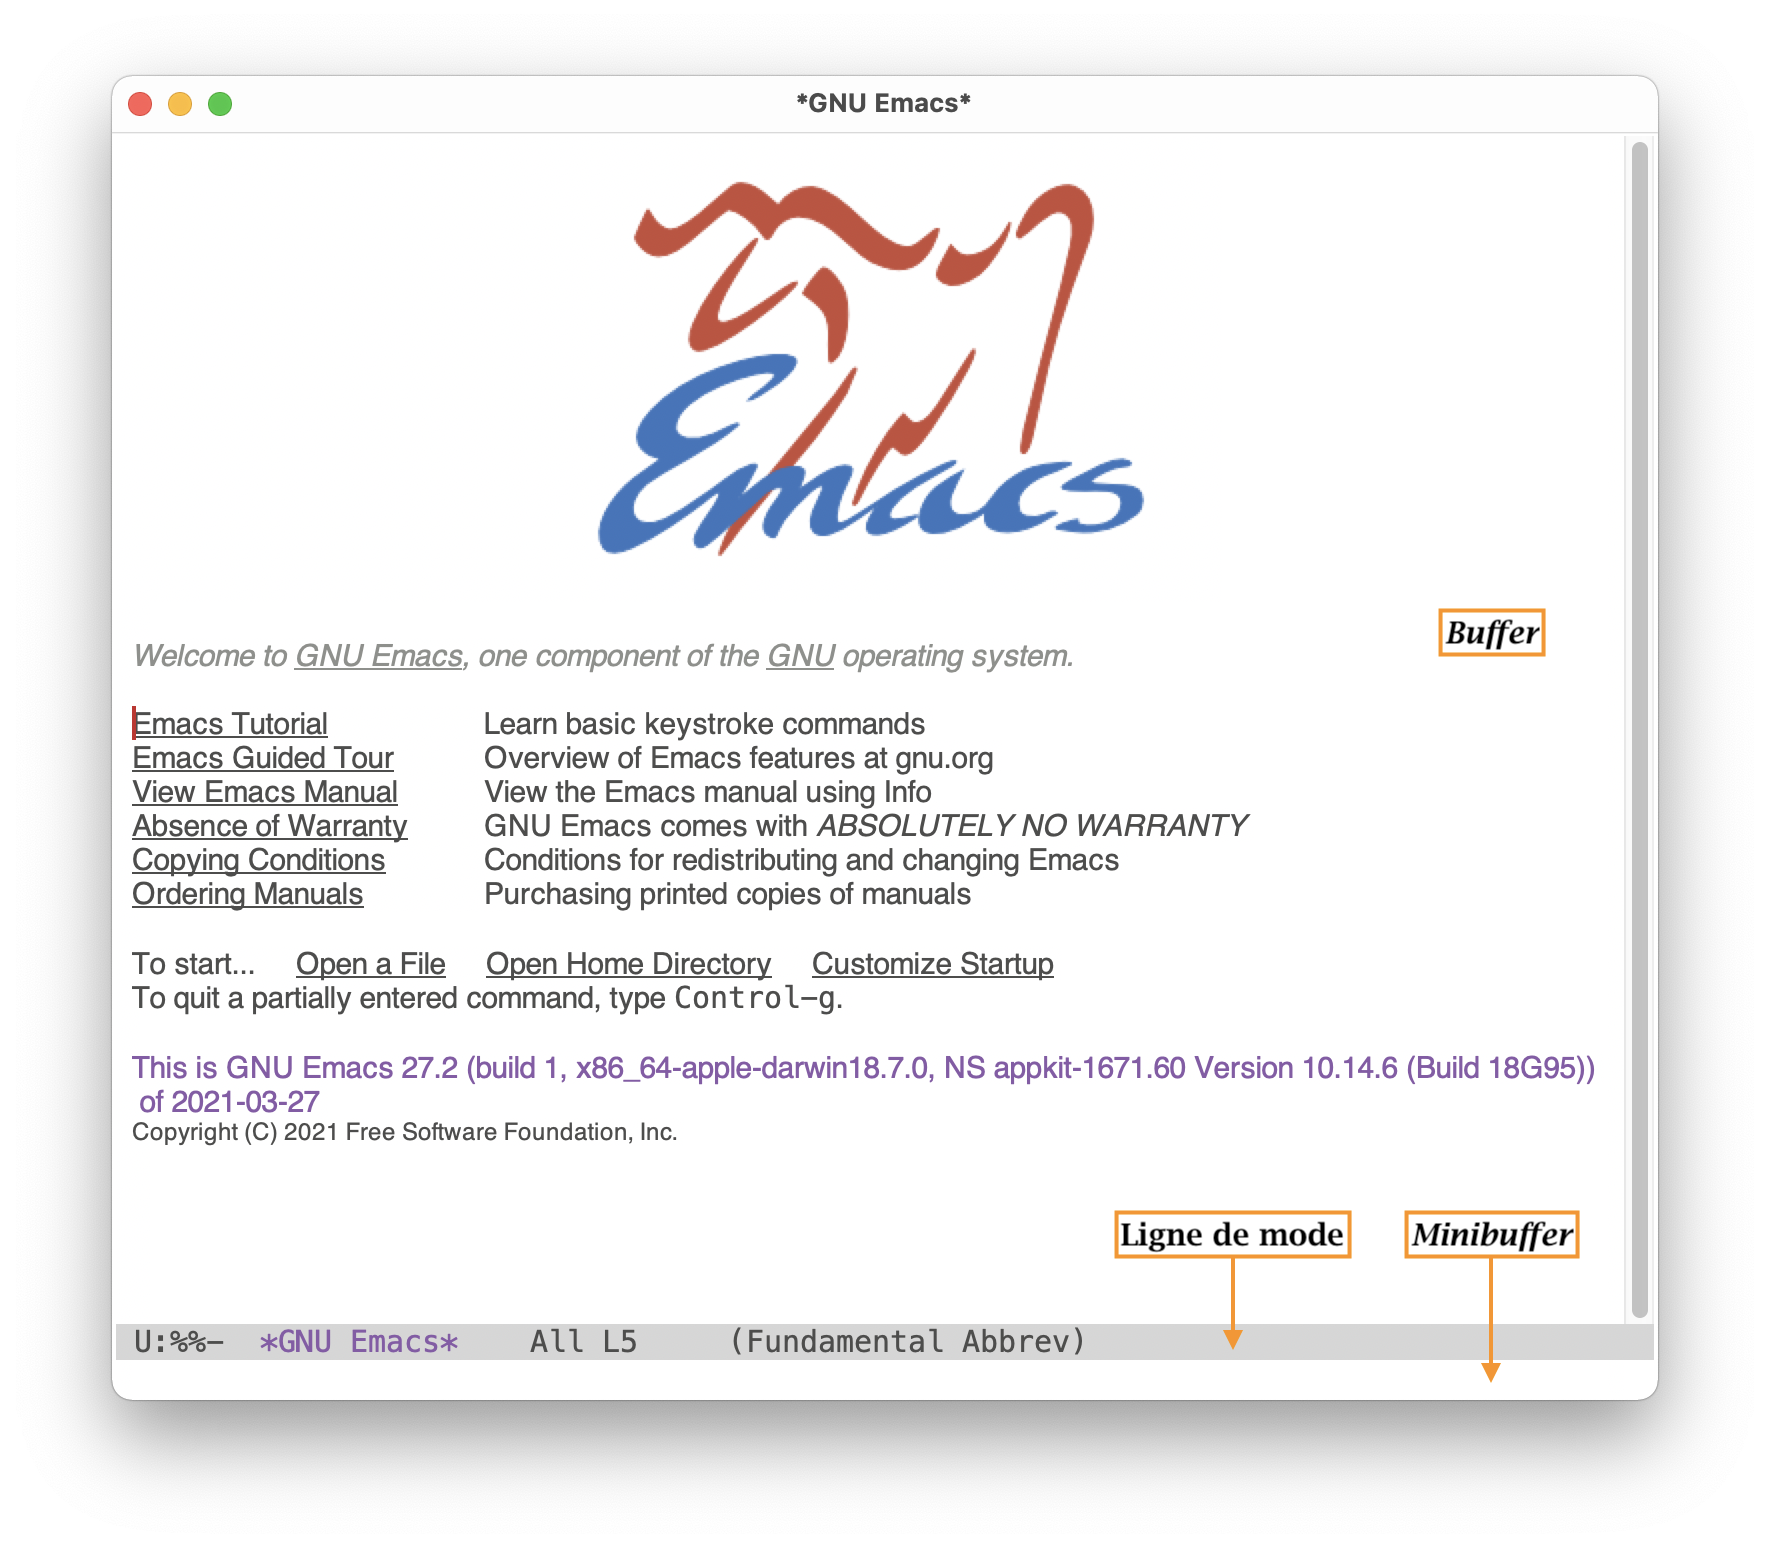
\includegraphics{images/emacswindow-screenshot}

  \begingroup
  \TPoptions{absolute=false}
  %% Identification de la barre de menu
  \begin{textblock}{0.35}(7.38,-6.58)
    \Large\faLongArrowAltRight
  \end{textblock}
  \begin{textblock}{1.75}(7.88,-6.59)
    \footnotesize\sffamily Barre de menu
  \end{textblock}

  %% Identification du buffer
  \begin{textblock}{0.35}(7.38,-3.38)
    \Large\faLongArrowAltRight
  \end{textblock}
  \begin{textblock}{1.75}(7.88,-3.39)
    \footnotesize\sffamily \emph{Buffer}
  \end{textblock}

  %% Identification de la mode line
  \begin{textblock}{0.35}(7.38,-0.28)
    \Large\faLongArrowAltRight
  \end{textblock}
  \begin{textblock}{1.75}(7.88,-0.29)
    \footnotesize\sffamily Ligne de mode
  \end{textblock}

  %% Identification du minibuffer
  \begin{textblock}{0.35}(7.38,-0.08)
    \Large\faLongArrowAltRight
  \end{textblock}
  \begin{textblock}{1.75}(7.88,-0.09)
    \footnotesize\sffamily \emph{Minibuffer}
  \end{textblock}
  \endgroup
  \caption[Fenêtre de GNU~Emacs sous macOS]{Fenêtre de GNU~Emacs et
    ses différentes parties au lancement de l'application sous macOS.
    Sous Windows et Linux, la barre de menu se trouve à l'intérieur de
    la fenêtre.}
  \label{fig:ess:emacswindow}
\end{figure}


\section{\emph{Emacs-ismes} et \emph{Unix-ismes}}
\label{sec:emacs+ess:ismes}

Emacs possède sa propre terminologie qu'il vaut mieux connaitre
lorsque l'on consulte la documentation. De plus, l'éditeur utilise des
conventions du monde Unix qui sont moins usitées sur les plateformes
Windows et macOS.

\begin{itemize}
\item Dans les définitions de raccourcis claviers:
  \begin{itemize}
  \item \code{C} est la touche \code{Contrôle} (\ctlkey);
  \item \code{M} est la touche \code{Meta}, qui correspond à la touche
    \code{Alt} de gauche sur un PC ou la touche \code{Option}
    (\optkey) sur un Mac (toutefois, voir l'encadré à la
    \autopageref{fig:ess:meta});
  \item \code{ESC} est la touche \code{Échap} (\esckey) et
    est équivalente à \code{Meta};
  \item \code{SPC} est la barre d'espacement;
  \item \code{DEL} est la touche \code{Retour arrière} (\delkey) ---
    \emph{et non la touche} \code{Supprimer}.
  \item \code{RET} est la touche \code{Entrée} (\returnkey);
  \end{itemize}
\item Toutes les fonctionnalités de Emacs correspondent à une commande
  qui peut être tapée dans le \emph{minibuffer}. \code{M-x} démarre
  l'invite de commande.
\item Le caractère \,\verb=~=\, représente le dossier vers lequel
  pointe la variable d'environnement \code{\$HOME} (Linux, macOS) ou
  \code{\%HOME\%} (Windows). C'est le dossier par défaut de Emacs.
\item La barre oblique (\code{/}) est utilisée pour séparer les
  dossiers dans les chemins d'accès aux fichiers, même sous Windows.
\item En général, il est possible d'appuyer sur \code{TAB} dans le
  \emph{minibuffer} pour compléter les noms de fichiers ou de
  commandes.
\end{itemize}

\begin{figure}[t]
  \refstepcounter{dummy}
  \label{fig:ess:meta}
  \begin{titled-frame}{Configuration de la touche Meta sous macOS}
    Par défaut sous macOS, la touche \code{Meta} est assignée à
    \code{Option} (\optkey). Sur les claviers français, cela empêche
    d'accéder à certains caractères spéciaux tels que {\og}[{\fg},
    «]», «\{» ou «\}».

    Une solution à cette fâcheuse situation consiste à assigner
    la touche \code{Meta} à \code{Commande} (\cmdkey). Cela bloque
    alors l'accès à certains raccourcis Mac, mais la situation est
    moins critique ainsi.

    Pour assigner la touche \code{Meta} à \code{Commande} (\cmdkey) et
    laisser la touche \code{Option} (\optkey) jouer son rôle usuel, il
    suffit d'insérer les lignes suivantes dans son fichier de
    configuration \code{.emacs} (voir la
    \autoref{sec:emacs+ess:configuration}):
\begin{verbatim}
(setq-default ns-command-modifier 'meta)
(setq-default ns-option-modifier 'none)
\end{verbatim}
  \end{titled-frame}
\end{figure}



\section{Commandes de base}
\label{sec:emacs+ess:commandes}

Emacs comporte une pléthore de commandes, il serait donc futile de
tenter d'en faire une liste exhaustive ici. Nous nous contenterons de
mentionner les commandes les plus importantes regroupées par tâche.

\subsection{Les essentielles}
\label{sec:emacs+ess:commandes:essentielles}

\begin{ttscript}{M-x}
\item[\code{M-x}] démarrer l'invite de commande
\item[\code{C-g}] bouton de panique: annuler, quitter! Presser plus
  d'une fois au besoin.
\end{ttscript}

\subsection{Manipulation de fichiers}
\label{sec:emacs+ess:commandes:fichiers}

Entre parenthèses, le nom de la commande Emacs correspondante. On peut
entrer cette commande dans le \emph{minibuffer} au lieu d'utiliser le
raccourci clavier.

\tipbox{Il n'existe pas de commande «nouveau
  fichier» dans Emacs. Pour créer un nouveau fichier, il suffit
  d'ouvrir un fichier qui n'existe pas déjà.\index{Emacs!nouveau fichier}}

\begin{ttscript}{C-x C-w}
\item[\code{C-x C-f}] ouvrir un fichier (\code{find-file})
\item[\code{C-x C-s}] sauvegarder
  (\code{save-buffer})\index{Emacs!sauvegarder}
\item[\code{C-x C-w}] sauvegarder sous
  (\code{write-file})\index{Emacs!sauvegarder sous}
\item[\code{C-x k}] fermer un fichier (\code{kill-buffer})
  \\[\baselineskip]
\item[\code{C-\_}] annuler (pratiquement illimité); aussi
  \code{C-x u} (\code{undo})
  \\
\item[\code{C-s}] recherche incrémentale avant
  (\code{isearch-forward})
\item[\code{C-r}] Recherche incrémentale arrière
  (\code{isearch-backward})
\item[\code{M-\%}] rechercher et remplacer
  (\code{query-replace})\index{Emacs!rechercher et remplacer}
\end{ttscript}


\subsection{Déplacements simples du curseur}
\index{Emacs!déplacement du curseur}
\label{sec:emacs+ess:commandes:deplacement}

\begin{ttscript}{C-DEL | C-w}
\item[\code{C-b} | \code{C-f}] déplacer d'un caractère vers
  l'arrière~|~l'avant \newline
  (\code{backward-char} | \code{forward-char})
\item[\code{C-a} | \code{C-e}] aller au début~|~fin de la ligne \newline
  (\code{move-beginning-of-line} | \code{move-end-of-line})
\item[\code{C-p} | \code{C-n}] aller à la ligne précédente~|~suivante \newline
  (\code{previous-line} | \code{next-line})
\item[\code{M-<} | \code{M->}] aller au début~|~fin du fichier \newline
  (\code{beginning-of-buffer} | \code{end-of-buffer})
  \\
\item[\code{DEL} | \code{C-d}] effacer le caractère à
  gauche~|~droite du curseur  \newline
  (\code{delete-backward-char} | \code{delete-char})
\item[\code{M-DEL} | \code{M-d}] effacer le mot à gauche~|~droite
  du curseur  \newline
  (\code{backward-kill-word} | \code{kill-word})
\item[\code{C-k}] supprimer jusqu'à la fin de la ligne (\code{kill-line})
\end{ttscript}

\osxbox{Plusieurs des raccourcis clavier de Emacs composés avec la
  touche \code{Contrôle} (\ctlkey) sont valides sous macOS. Par
  exemple, \ctlkey\,\code{A} et \ctlkey\,\code{E} déplacent le curseur
  au début et à la fin de la ligne dans les champs texte.}


\subsection{Sélection de texte, copier, coller, couper}
\index{Emacs!sélection}
\label{sec:emacs+ess:commandes:selection}

\begin{ttscript}{C-x C-w}
\item[\code{C-SPC}] débute la sélection (\code{set-mark-command})
\item[\code{C-w}] couper la sélection (\code{kill-region})
\item[\code{M-w}] copier la sélection (\code{kill-ring-save})
\item[\code{C-y}] coller (\code{yank})
\item[\code{M-y}] remplacer le dernier texte collé par la
  sélection précédente \newline
  (\code{yank-pop})
\end{ttscript}

\tipbox{Il est possible d'utiliser les raccourcis clavier usuels de
  Windows (\code{C-c}, \code{C-x}, \code{C-v}) et macOS
  (\cmdkey\,\code{C}, \cmdkey\,\code{X}, \cmdkey\,\code{V}) en
  activant le mode CUA dans le menu \code{Options}.}

\windowsbox{ On peut copier-coller directement avec la souris dans Windows en
  sélectionnant du texte puis en appuyant sur le bouton central (ou la
  molette) à l'endroit souhaité pour y copier le texte.}


\subsection{Manipulation de fenêtres}
\label{sec:emacs+ess:commandes:fenetres}

\begin{ttscript}{C-x C-w}
\item[\code{C-x b}] changer de \emph{buffer}
  (\code{switch-buffer})
\item[\code{C-x 2}] séparer l'écran en deux fenêtres
  (\code{split-window-vertically})
\item[\code{C-x 1}] conserver uniquement la fenêtre courante \newline
  (\code{delete-other-windows})
\item[\code{C-x 0}] fermer la fenêtre courante
  (\code{delete-window})
\item[\code{C-x o}] aller vers une autre fenêtre lorsqu'il y en a
  plus d'une \newline
  (\code{other-window})
\end{ttscript}

\subsection{Manipulation de fichiers de script dans le mode ESS}
\index{Emacs!mode ESS|(}
\label{sec:emacs+ess:commandes:script}

Le mode ESS dispose de fonctions «intelligentes» qui facilitent
grandement la manipulation des fichiers de script. Les deux
principales commandes à connaitre sont les suivantes:
\begin{ttscript}{C-x C-w}
\item[\code{C-RET}] évaluer dans le processus R la ligne sous le
  curseur ou la région sélectionnée, puis déplacer le curseur à la
  prochaine expression \newline
  (\code{ess-eval-region-or-line-and-step})
\item[\code{C-c C-c}] évaluer dans le processus R la région
  sélectionnée, la fonction ou le paragraphe (tout bloc entre deux
  lignes blanches) dans lequel se trouve le curseur, puis déplacer le
  curseur à la prochaine expression \newline
  (\code{ess-eval-region-or-function-or-paragraph-and-step})
\end{ttscript}
Les quelques autres fonctions utiles sont:
\begin{ttscript}{C-x C-w}
\item[\code{\_}] insérer le symbole d'affectation \verb*| <- | (sauf
  dans les champs texte et dans les commentaires);
  appuyer deux fois consécutives pour obtenir le caractère de
  soulignement \newline
  (\code{ess-smart-S-assign})
\item[\code{C-c C-z}] déplacer le curseur vers le processus R \newline
  (\code{ess-switch-to-inferior-or-script-buffer})
\item[\code{C-c C-f}] évaluer le code de la fonction courante dans
  le processus R \newline
  (\code{ess-eval-function})
\item[\code{C-c C-l}] évaluer le code du fichier courant en entier dans
  le processus R \newline
  (\code{ess-load-file})
\item[\code{C-c C-v}] aide sur une commande R
  (\code{ess-display-help-on-object})
\end{ttscript}

\subsection{Interaction avec l'invite de commande R}
\label{sec:emacs+ess:commandes:invite}

\begin{ttscript}{M-p |M-n}
\item[\code{M-p} | \code{M-n}] commande précédente~|~suivante
  dans l'historique \newline
  (\code{previous-matching-history-from-input} | \newline
  \code{next-matching-history-from-input})
\item[\code{C-c C-z}] déplacer le curseur vers le fichier de script
  courant \newline
  (\code{ess-switch-to-inferior-or-script-buffer})
\item[\code{M-h}] sélectionner le résultat de la dernière commande \newline
  (\code{mark-paragraph})
\item[\code{C-c C-o}] effacer le résultat de la dernière commande \newline
  (\code{comint-delete-output})
\item[\code{C-c C-v}] aide sur une commande R
  (\code{ess-display-help-on-object})
\item[\code{C-c C-q}] terminer le processus R (\code{ess-quit})
\end{ttscript}

\subsection{Consultation des rubriques d'aide de R}
\label{sec:emacs+ess:commandes:aide}

\begin{ttscript}{m, m}
\item[\code{p} | \code{n}] aller à la section précédente~|~suivante de
  la rubrique \newline
  (\code{ess-skip-to-previous-section} |
  \code{ess-skip-to-next-section})
\item[\code{s a}] aller à la section de la liste des arguments \emph{(Arguments)}
\item[\code{s D}] aller à la section des détails sur la fonction \emph{(Details)}
\item[\code{s v}] aller à la section sur la valeur retournée par la
  fonction \emph{(Value)}
\item[\code{s s}] aller à la section des fonctions apparentée \emph{(See Also)}
\item[\code{s e}] aller à la section des exemples \emph{(Examples)}
\item[\code{l}] évaluer la ligne sous le curseur; pratique pour
  exécuter les exemples \newline
  (\code{ess-eval-line-and-step})
\item[\code{r}] évaluer la région sélectionnée (\code{ess-eval-region})
\item[\code{h}] ouvrir une nouvelle rubrique d'aide, par défaut pour
  le mot se trouvant sous le curseur
  (\code{ess-display-help-on-object})
\item[\code{q}] retourner au processus ESS en laissant la rubrique
  d'aide visible \newline
  (\code{ess-switch-to-end-of-ESS})
\item[\code{x}] fermer la rubrique d'aide et retourner au processus
  ESS \newline
  (\code{ess-kill-buffer-and-go})
\end{ttscript}



\section{Anatomie d'une session de travail (ter)}
\label{sec:emacs+ess:session}

On reprend ici la description de la type présentée à la
\autoref{sec:presentation:session}, mais en expliquant comment
compléter chaque étape dans Emacs avec le mode ESS. Sont intercalés
dans les instructions les raccourcis clavier des commandes Emacs et
les accès par les menus, le cas échéant.

\begin{enumerate}
\item Lancer Emacs et ouvrir un fichier de script.
  \begin{trivlist}
  \item
    \makebox[0.28\linewidth][l]{%
      \colorbox{codebg}{\code{C-x C-f}}}
    \hfill
    \makebox[0.68\linewidth][l]{%
      \colorbox{codebg}{\code{File|Open File...}}}
  \end{trivlist}
  En spécifiant un nom de fichier qui n'existe pas déjà, on crée un
  nouveau fichier de script. S'assurer de terminer le nom du nouveau
  fichier par \code{.R} pour que Emacs reconnaisse automatiquement
  qu'il s'agit d'un fichier de script R.
\item Démarrer un processus R à l'intérieur de Emacs.
  \begin{trivlist}
  \item
    \makebox[0.28\linewidth][l]{%
      \colorbox{codebg}{\code{M-x R }\returnkey}}
  \end{trivlist}
  Emacs demandera de spécifier de répertoire de travail
  (\emph{starting data directory}). Accepter la valeur par défaut ou
  indiquer un autre dossier.
  \begin{trivlist}
  \item
    \makebox[0.28\linewidth][l]{%
      \colorbox{codebg}{\code{\textasciitilde/ = }\returnkey}}
  \end{trivlist}
  Un éventuel message de Emacs à l'effet que le fichier
  \code{.Rhistory} n'a pas été trouvé est sans conséquence et peut
  être ignoré.
\item Composer le code. Lors de cette étape, on se déplacera souvent
  du fichier de script à la ligne de commande afin d'essayer diverses
  expressions. On exécutera également des parties seulement du code se
  trouvant dans le fichier de script. Les commandes les plus utilisées
  sont alors:
  \begin{trivlist}
  \item
    \makebox[0.28\linewidth][l]{%
      \colorbox{codebg}{\code{C+RET}}}
    \hfill
    \makebox[0.68\linewidth][l]{%
      \colorbox{codebg}{\code{ESS|Eval region | line}}}
  \item
    \makebox[0.28\linewidth][l]{%
      \colorbox{codebg}{\code{C-c C-c}}}
    \hfill
    \makebox[0.68\linewidth][l]{%
      \colorbox{codebg}{\code{ESS|Eval region | func | para \& step}}}
  \item
    \makebox[0.28\linewidth][l]{%
      \colorbox{codebg}{\code{C-c C-z}}}
    \hfill
    \makebox[0.68\linewidth][l]{%
      \colorbox{codebg}{\code{ESS|Process|Switch to process buffer}}}
  \end{trivlist}
\item Sauvegarder le fichier de script.
  \begin{trivlist}
  \item
    \makebox[0.28\linewidth][l]{%
      \colorbox{codebg}{\code{C-x C-s}}}
    \hfill
    \makebox[0.68\linewidth][l]{%
      \colorbox{codebg}{\code{File|Save}}}
  \end{trivlist}
  Les quatrième et cinquième caractères de la ligne de mode changent
  de \,\verb|**|\, à \,\verb|--|.
\item Sauvegarder si désiré l'espace de travail de R avec
  \code{save.image()}\index{save.image@\code{save.image}}. Cela n'est
  habituellement pas nécessaire à moins que l'espace de travail ne
  contienne des objets importants ou longs à recréer.
\item Quitter le processus R.
  \begin{trivlist}
  \item
    \makebox[0.28\linewidth][l]{%
      \colorbox{codebg}{\code{C-c C-q}}}
    \hfill
    \makebox[0.68\linewidth][l]{%
      \colorbox{codebg}{\code{iESS|Quit}}}
  \end{trivlist}
  Cette commande de ESS se charge de fermer tous les fichiers associés
  au processus R. On peut ensuite quitter Emacs en fermant
  l'application de la manière usuelle.
\end{enumerate}
\index{Emacs!mode ESS|)}

\videobox{\link{https://youtu.be/KtmFDm2AKM4}{Anatomie d'une session de travail
    avec GNU Emacs}}{%
  La session de travail type avec GNU Emacs ci-dessus fait aussi l'objet
  d'\link{https://youtu.be/KtmFDm2AKM4}{une vidéo}.}


\section{Configuration de l'éditeur}
\label{sec:emacs+ess:configuration}

Une des grandes forces de Emacs est qu'à peu près chacune de ses
facettes est configurable: couleurs, polices de caractère, raccourcis
clavier, etc.

La configuration de Emacs repose sur des commandes réunies dans un
nommé \code{.emacs} (le point est important!) que Emacs lit au
démarrage. Le fichier \code{.emacs} doit se trouver dans le dossier
\,\verb=~/=, c'est-à-dire dans le dossier de départ de l'utilisateur
sous Linux et macOS, et dans le dossier référencé par la variable
d'environnement \code{\%HOME\%} sous Windows.

\videobox{\link{https://youtu.be/jdtjBBkfhO0}{Création de fichiers de
    configuration pour Emacs et R}}{%
  Visionnez la vidéo portant sur la
  \link{https://youtu.be/jdtjBBkfhO0}{création de fichiers de
    configuration} pour Emacs et R.}


\section{Aide et documentation}
\label{sec:emacs+ess:aide}

Emacs possède son propre système d'aide très exhaustif, mais dont la
navigation est peu intuitive selon les standards d'aujourd'hui.
Consulter le menu \code{Help}.

Autrement, on trouvera dans les sites respectifs des deux projets les
manuels de \link{https://www.gnu.org/software/emacs}{Emacs} et de
\link{https://ess.r-project.org}{ESS}.

Enfin, si le désespoir vous prend au cours d'une séance de codage
intensive, vous pouvez toujours consulter le psychothérapeute Emacs.
On le trouve, bien entendu, dans le menu \code{Help}!

\index{Emacs|)}

%%% Local Variables:
%%% mode: latex
%%% TeX-engine: xetex
%%% TeX-master: "programmer-avec-r"
%%% coding: utf-8
%%% End:
